\documentclass[tikz]{standalone}

\usepackage{amsmath}
\usetikzlibrary{positioning}

\begin{document}
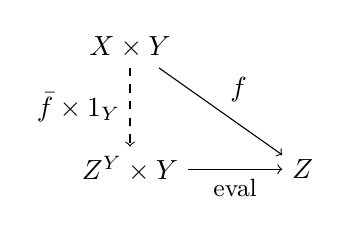
\begin{tikzpicture}
	\node (XY) {$X\times Y$};
	\node [below=1.0cm of XY] (ZYY) {$Z^Y\times Y$};
	\node [right=1.2cm of ZYY] (Z) {$Z$};
	\draw [->] (XY) to node [above right] {$f$} (Z);
	\draw [->, dashed] (XY) to node [left] {$\bar{f}\times 1_Y$} (ZYY);
	\draw [->] (ZYY) to node [below] {\small$\operatorname{eval}$} (Z);
\end{tikzpicture}
\end{document}
